\chapter{Internship report}
\section{Week 1}
\subsection{Company profile}
The first two days of the week were spent getting to know all colleagues and familiarize myself with internal processes and guidelines. Zurich is the headquarters of Enclustra GmbH and therefore the majority of hardware and software design is being done here. Around forty people, most of which are hardware and software engineers, work in the Zurich office. The company itself is divided into two areas, \ac{FPGA} Design Center and \ac{FPGA} Solution Center.
The former is offering customer-specific design services implementing applications on \acp{FPGA} and providing support and custom \ac{IP} components. Areas of expertise include wired networks and switching, wireless communications (\ac{SDR}), smart cameras, embedded interfaces (\ac{PCIe}, \ac{USB}, \ac{AXI}, ethernet, etc.), test and measurement (sensors, data acquisition, \ac{DSP}) and drive/motion control. 
The latter designs custom \ac{FPGA}/\ac{SoC} modules and \ac{IP} solutions. Several base board families and \ac{FPGA} module families are developed and supported which can be adapted to the needs of the application by offering different performance key points. Reference designs for each combination of base board and module are provided as a starting point for customers.
\subsection{Market research}
Furthermore, my task was to do market research on artificial intelligence and artificial intelligence on \acp{FPGA} especially. The four key platforms for artificial neural network applications are shown in~\ref{fig:overview}.
\begin{figure}[!htb]
	\centering
		\includegraphics[width=0.75\textwidth]{bilder/overview.png}
		\caption{Hardware platform overview}
		\label{fig:overview}
\end{figure}
A qualitative design trade-off is shown on the $x$- and $y$-axis in terms of power efficiency and performance versus flexibility and ease-of-use. As Enclustras focus is on the embedded market, the market survey has been mainly on \acp{GPU}, \acp{FPGA} and \acp{ASIC} as full blown \acp{CPU} are too inefficient for embedded applications. Possible competitors as well as toolkits provided by \ac{FPGA} manufacturers such as Intel, Xilinx and Lattice have been evaluated. The results have been presented in a meeting in which a discussion has been held, where Enclustras products and services can fit. One of the results was to start planning an \ac{AI} demonstrator using Enclustra hardware. The purpose of this demonstrator was to showcase machine learning applications running on Enclustra hardware. As a preliminary step it was decided to check the Xilinx \ac{DNNDK} samples on an evaluation board, the ZCU 104.

\section{Week 2}
\subsection{Out-of-box testing}
At the beginning of the week a task unrelated to \ac{AI} was given to check upon internal documentation and customer support. Together with another recently hired employee, a day of out-of-box testing was scheduled. An Enclustra base board (Mercury+ PE1-400) together with a fitting \ac{FPGA} module (Mercury+ XU1) featuring a Xilinx \ac{MPSoC}.
Some details will be given for this specific \ac{FPGA} family as the Zynq-7000 \ac{SoC} and the Zynq-\ac{MPSoC} Xilinx product family are unique in the way dedicated ARM processors are combined with traditional \acp{FPGA}. A high level overview is shown in figure~\ref{fig:zynq-overview}.
\begin{figure}[!htb]
	\centering
		\includegraphics[width=\textwidth]{bilder/ZYNQ-overview.png}
		\caption{High level ZYNQ family overview~\cite{zynq-book}}
		\label{fig:zynq-overview}
\end{figure}
It shows the difference between traditional \acp{FPGA} and the Zynq product family. The main benefit here is the division between \ac{PS} and \ac{PL}. This allows to combine the benefits of traditional processing units with the flexibility of \acp{FPGA}. Custom logic and all peripheral devices can be implemented in the \ac{PL} part, while system control and even complete \acp{OS} (such as embedded Linux) can be done in the \ac{PS}. As this system is completely integrated in one package, the communication between the two fabrics is extremely fast and can be done using \ac{AXI} interfaces. The \ac{MPSoC} family even integrates several different types of processing units, \acp{APU}, \acp{GPU}, \acp{VPU} and \acp{RPU}.
The Enclustra module uses an \ac{MPSoC} Xilinx FPGA and our task was to go through the whole process of bringing up the base board together with a corresponding module to test customer experience using the provided documentation, user manual and reference design. The goal was to find unclear instructions in the documentation and provide feedback as to the overall experience bringing up the hardware out-of-the-box. First, the hardware reference design was loaded in the Vivado Design Suite and the bit stream generated. After, the hardware description file was exported so it can be used using the Xilinx \ac{SDK}. This allows to create applications in C/C++ against the custom hardware design. All of the provided sample applications have been tested and verified. Some unclear instructions were identified and discussed with the employee in charge to improve customer experience.
\subsection{Wiki updates and ZCU 104 testing}
The rest of the week was spend updating the internal Wiki page for \ac{AI}. Furthermore, the \ac{DNNDK} sample applications were tested on the ZCU 104 evaluation board. The provided examples include several state-of-the-art neural networks demonstrating key applications for neural network inference, such as image classification, face detection, object detection and pose detection. As only the image classification example worked directly for this particular evaluation a fix needed to be found. Another task was to introduce the topic of \ac{AI} to the whole company as \acp{ANN} was a completely new design field for a majority of the technical staff. Two PowerPoint presentations should be prepared, namely 'Introduction to \ac{AI}' and 'Introduction to \ac{ML} on \acp{FPGA}'. I started with the preparation of the first one in parallel with finding a bug fix for the other \ac{DNNDK} sample applications, as these should be part of the second presentation.

\section{Week 3}
The main focus of this week was research and starting to layout the first presentation. It was assumed that the audience is technology savvy but has no particular background in \ac{AI}. Thus, the presentation had to introduce the whole field and key concepts that enabled the rise of \ac{AI} applications in recent years. The first draft of the presentation was discussed in a meeting and some changes were made to the overall structure, the content and the degree of complexity.The rough structure of the presentation is as follows:
\begin{itemize}
	\item \textbf{Motivation}: To get the viewers interest it was shown that \ac{AI} applications are already part of daily life for everyone. This was achieved by showing that all of the major companies such as Google, Apple, Facebook, Microsoft as well as Tesla, Netflix and Amazon use \ac{AI} in their datacenters and products and allocate huge resources to \ac{AI} research. The importance of \ac{AI} was further enhanced by showing the rapid growth of annually published \ac{AI} papers and startups developing \ac{AI} systems. The trend from 1995 to 2015 resembles almost exponential growth in \ac{AI} research and products.
	\item \textbf{Definition}: As \ac{AI} has become such a buzz word in media a definition of the term was needed and what part of \ac{AI} is actually used in all of the common applications. \ac{ANN} that perform typical computer vision and language processing tasks are all part of \ac{ML}, which is a subset of \ac{AI}. \ac{ML} itself can then be divided into further subsets using roughly three learning methods, supervised learning, unsupervised learning and reinforcement learning. As supervised learning is the most commonly used method, the presentation focused on this method used to train \ac{ANN}. Furthermore, the different parts that comprise a \ac{ANN} are introduced, namely the neuron and how neurons are formed into layers. These layers are then stacked together to form an \ac{ANN}.
	\item \textbf{Key concepts}: An explanation of supervised learning was given with two distinct examples, linear regression and deep learning neural networks to illustrate the idea behind supervised learning: predict a value $y$ given an input $x$ by deploying a function $f(x)$. This function $f(x)$ is acquired by deploying a learning algorithm and usage of a so called training set, consisting of input pairs $x$ and $y$. The concept of inference and training were also explained with an emphasis on inference. Once a network is trained, only inference needs to be run, so this is the crucial part application wise.
\begin{figure}[!htb]
	\centering
		\includegraphics[width=\textwidth]{bilder/ilsvrc.png}
		\caption{ILSVRC winners}
		\label{fig:ilsvrc}
\end{figure}
	\item \textbf{Deep Learning}: Figure~\ref{fig:ilsvrc} shows the winners of the state-of-the-art ImageNet Large Scale Visual Recognition Challenge. It illustrates that the breakthrough in performance came not only from more sophisticated networks, but mainly from stacking different kinds of layers deeply, hence the name. The presentation was ended with the question, what hardware is best suited for \ac{ANN} applications. This question would be addressed in the second presentation 'Introduction to \ac{ML} on \acp{FPGA}'.
\end{itemize}
Alongside preparing the presentation the error preventing the more sophisticated examples was identified as the board crashed while performing tasks related to video analysis (face detection, pose detection, etc.). At first, it was suspected there were some problems with heat management and using the system monitor the temperature of the \ac{FPGA} was investigated during operation. As this seemed to be well within allowed borders specified by the Xilinx data sheet, other causes had to be found.

\section{Week 4}
\subsection{Presentation 'Introduction to \acs{AI}'}
At the beginning of the week the first presentation 'Introduction to \ac{AI}' was held before the technical stuff of the company. The general background and principles of \ac{ML} have been introduced and an outlook given to the second presentation, which would go more into detail about the actual hardware realization. 
\subsection{Xilinx Vivado and \acs{DNNDK} workflow}
The rest of the week was spent going through various tutorials provided by Xilinx to familiarize myself with the workflow and the \ac{DNNDK} toolkit. As the state of tools used for \ac{AI} applications on \ac{FPGA} is still in flux, several approaches needed to be evaluated:
\begin{itemize}
	\item \textbf{\ac{DNNDK} workflow}: Version 2.08 of the toolkit supported only the Caffe neural network training framework and needs a network description file and the trained weights as input. The key component here is the \ac{DPU} \ac{IP} core provided by the \ac{DNNDK} toolkit. This core is integrated via Vivado into the block design of the hardware and can be configured and adjusted for several performance and power profiles.
	\item \textbf{\ac{DNNDK} \ac{SDSoC}}: Another option is to abstract away the whole Vivado block design process and use Xilinx \ac{SDSoC} to implement the whole system in a higher programming language, C++. Supported functions can then be flagged as being executed in the \ac{PL} part of the system. This approach makes using a traditional \ac{HDL} obsolete and is deemed more accessible. This approach uses the established Xilinx reVision stack for development providing high level \acp{API} for computer vision.
\end{itemize}
Furthermore, the \ac{IP} core provided by the \ac{DNNDK} toolkit was studied in more detail. A new base board was in the production state phase and the idea was to have a \ac{ML} design ready to showcase the capabilities of the new board.
\begin{figure}[!htb]
	\centering
		\includegraphics[width=\textwidth]{bilder/DPU_example_design.png}
		\caption{Example system with integrated \acs{DPU} \cite[p.~8]{dpu}}
		\label{fig:dpu_example}
\end{figure}
Figure~\ref{fig:dpu_example} shows an example hardware design with integrated \ac{DPU} module. In this example a camera is connected via the \ac{MIPI} \ac{CSI2} interface to the \ac{PS}. \ac{DMA} is usually used in conjunction with an \ac{AXI} interconnect to communicate with the \ac{PS}. The captured images are used as the input to the neural network and the \ac{DPU} itself can be viewed as a co-processor to the \ac{PS} implemented in the \ac{PL} fabric. The \ac{IP} core itself is customizable and the number of \ac{DPU} processor units, the size of the \ac{DPU} and the usage of \ac{DSP} blocks among other parameters are configurable. The decision on which size to use is based upon the performance demands of the application.

\section{Week 5}
\subsection{Presentation 'Introduction to \ac{ML} on \acp{FPGA}'}
In this week I started working on the second presentation 'Introduction to \ac{ML} on \acp{FPGA}'. This time the focus should be on the hardware needed to handle typical \ac{ML} workloads, namely inference and training along all major fields of applications where \ac{ANN} are used. The main areas are: image classification, object detection, semantic segmentation, optical character recognition and speech recognition. The presentation structure is as follows:
\begin{itemize}
	\item \textbf{\ac{ANN} workload:} Using a state-of-the-art neural network (resnet50) the number of operations per image were illustrated to show the vast amount of compute and memory needed for a single image. This was done for inference and training respectively with the purpose of driving home the challenges involved in \ac{ML} applications. Moreover, the majority of operations are costly \ac{MAC} operations which take several clock cycles to complete.
	\item \textbf{Hardware for training:} The industry right now in terms of \ac{ANN} training is dominated by NVIDIA and so the clear answer here was \ac{GPU}. There are a number of start-ups developing alternative solutions to get into the \ac{ANN} training market. The main advantage these start-ups have is that they can design from scratch and use an architecture tailored to the specific requirements of \ac{ANN} training. The sheer number of floating point 32 operations and the requirements for memory are strictly not suited for \acp{FPGA}.
	\item \textbf{Hardware for inference:} The picture is different for inference. Here, a lot of research has been done in using quantization and pruning of \ac{ANN} models without impeding the performance of these networks. The reason for this is, that neural networks are inherently over-parametrized and this is necessary for the training algorithms to work. Once a trained network is obtained however, the network can be compressed severely (up to 90 \%) without network degradation. A qualitative comparison of the available platforms was made to show the strengths and weaknesses of each platform. The flexibility of \acp{FPGA} make them a suitable platform for \ac{ANN} inference.
	\item \textbf{\ac{FPGA} architecture:} Figure~\ref{fig:fpga_arch} shows the two possible high-level architectures that are typically used in neural network implementations. On the left you have the streaming architecture where basically the structure of the neural network is mirrored by the hardware implementation. The main benefit is the efficiency and customizability as the hardware can be tailored specifically to each network. The other approach is shown on the right. This is a more general approach in that it has a single computation engine which breaks down the operations needed for neural network inference. These operations are controlled by a host and executed on demand. The main benefit here is the flexibility. As the types of layers in a neural network are fixed, efficient implementation of these different types of layers enables the deployment of arbitrary neural networks. The downside is that the implementation is limited by the architecture in terms of tailoring the hardware implementation to the neural network.
	\begin{figure}[!htb]
	\centering
		\includegraphics[width=\textwidth]{bilder/FPGA_arch.png}
		\caption{\acs{FPGA} architecture overview}
		\label{fig:fpga_arch}
\end{figure}
	\item \textbf{\ac{DNNDK} work flow:} Lastly, the \ac{DNNDK} work flow is introduced with a focus on adjusting the \ac{DPU} \ac{IP} core to custom boards. Some demonstrations implemented on the ZCU 104 evaluation board were used to finish the presentation and show the employees, what is possible with the tools available.
\end{itemize}
\subsection{Xilinx \acs{ML} event Munich}
In this week on Thursday there was a Xilinx \ac{ML} seminar in Munich, where I went to with my supervisor to get more information about Xilinx \ac{AI} solutions. This was a whole day event with several segments, showing off the capabilities and the work flow of Xilinx cloud and edge \ac{AI} tools. This was also a great opportunity for networking and speaking in person to top Xilinx \ac{FAE} engineers.

\section{Week 6}
\subsection{Xilinx \acs{ML} event report}
All of the new information gathered at the Xilinx seminar last week needed to be transferred to the internal Wiki and properly documented. 
Three main tasks were worked upon in this week, namely preparing the second presentation 'Introduction to \ac{ML} on \ac{FPGA}', getting all of the \ac{DNNDK} sample applications to work on the ZCU 104 evaluation board and evaluating a possible collaboration with an ETH start-up called Synthara.
\subsection{Presentation 'Introduction to \ac{ML} on \acp{FPGA}'}
Extensive market research has been conducted to find resources and ideas on how to present the different hardware platforms. The difficulty lies therein, that there are no standardized performance metrics for neural networks. Performance is strongly dependent on the network used and the individual use case. This leads to a lot of unfair comparisons, both in research and industry when numbers are shown. Therefore, a qualitative approach was chosen as doing all of these comparisons would have taken an extreme amount of work time and effort, requiring special hardware as well.
\subsection{Bugfix for ZCU 104 evaluation board}
After reading through a vast amount of documentation and employing the help of online resources, mainly the Xilinx official forums, a solution was found to the problem. It turned out to be a specific problem of the ZCU 104 evaluation board which made it hard to track down. The solution to this was provided by an unofficial patch by on e of the Xilinx employees online. The board has power issues when running at full load resulting in the already mentioned problem of freezing the board in the middle of running the sample applications. After applying the patch all of the sample applications worked. These included image classification with resnet50 and inception-v1 as well as real time face detection, object detection and pose detection using other popular \ac{ANN}
\subsection{Synthara collaboration}
During research for neural network accelerator implementations I read about an ETH start-up providing this service in the form of an \ac{ASIC}. However, their prototypes as a proof-of-concept are implemented on \acp{FPGA}. Thus, we reached out to them and scheduled a meeting. During this meeting we discussed the possibility of a cooperation. The idea was to implement a demonstrator for the Embedded World 2020 conference showing off Enclustra hardware and using the Synthara neural network accelerator. The demo is a game of rock-paper-scissors played by a human player against a robotic hand. The setup can be seen in figure~\ref{fig:demonstrator}. The robot hand is controlled via \ac{USB} using \ac{PWM} to control each finger individually. The human players movement is captured by a camera connected via \ac{MIPI} to the \ac{FPGA} board. The \ac{FPGA} handles all image preprocessing and is running a custom neural network capable of detecting hand gestures. The control signals for the robot hand are also given by the FPGA.
	\begin{figure}[!htb]
	\centering
		\includegraphics[width=\textwidth]{bilder/demonstrator.png}
		\caption{Rock-paper-scissors demonstrator setup}
		\label{fig:demonstrator}
	\end{figure}

\section{Week 7}
\subsection{Presentation 'Introduction to \ac{ML} on \acp{FPGA}'}
At the beginning of the week I held the second presentation 'Introduction to \ac{ML} on \acp{FPGA}' in front of the assembled engineering employees. At the end of the presentation a live demonstrator was shown at my work place. The ZCU 104 was used as the platform to show off all of the \ac{ML} examples provided by the \ac{DNNDK} and upcoming questions answered. 
\subsection{Vivado hardware design and embedded \acs{OS}}
The rest of the week was spent doing in depth research on integrating \ac{MIPI} into a Vivado block design. The reason for this is that Enclustra developed a new base board, the Mars ST3. This board features a \ac{MIPI} \ac{CSI} connector allowing high-speed video streaming with up to four lanes and a bit rate of 2.5 Gbit/s per lane (or 2.9 Gbit/s depending on the chosen clock rate). The camera chosen was the Raspberry Pi camera with a SONY image sensor. As \ac{MIPI} is not an open standard, research has been conducted into open source implementations of interfacing with the \ac{MIPI} protocol. After discussing the open source alternatives with more experienced employees, those solutions were deemed unsuitable for the task at hand. The alternative solution is to use a Xilinx \ac{IP} core which is available as a time limited evaluation license. The starting point was the ZCU 104 reference design, which included the whole \ac{MIPI} \ac{IP} core design. It consists of two main parts, the \ac{MIPI} D-PHY and the \ac{MIPI} Tx/Rx subsystem
\begin{figure}[!htb]
	\centering
		\includegraphics[width=\textwidth]{bilder/MIPI_dphy.png}
		\caption{D-PHY \acs{MIPI} \acs{IP} core overview~\cite{mipi-dphy}}
		\label{fig:mipi_dphy}
\end{figure}
A high-level view of the Xilinx \ac{MIPI} D-PHY \ac{IP} core system is shown in figure~\ref{fig:mipi_dphy}. The communication takes place between a Master and Slave with one clock lane and up to 4 data lanes. This \ac{IP} core allows proper communication on this high-speed I/O interface standard. The complete receiver subsystem is shown in figure~\ref{MIPI_rx}.
\begin{figure}[!htb]
	\centering
		\includegraphics[width=\textwidth]{bilder/MIPI_rx.png}
		\caption{Receiver \acs{MIPI} \acs{IP} core subsystem~\cite{mipi-rx}}
		\label{fig:mipi_dphy}
\end{figure}
The D-PHY \ac{IP} core is part of this subsystem and in combination with the rest of the Rx subsystem allows the integration of a \ac{MIPI} based image sensor and an image sensor pipe. The captured images can then be accessed via \ac{AXI} interfaces. This part of the system needed to be integrated into the complete hardware design in Vivado consisting of the ZYNQ \ac{MPSoC}, the \ac{DPU} \ac{IP} core and the usual peripheral interfaces (\ac{USB}, DisplayPort, HDMI, etc.). On top of that, an embedded Linux \ac{OS} needed to be built to control the applications and provide a working demonstration environment. The chosen Linux distribution for this task was the Xilinx supported Petalinux, which is itself based on Yocto.

\section{Week 8}
\subsection{Vivado hardware design and embedded \acs{OS}}
\begin{figure}[!htb]
	\centering
		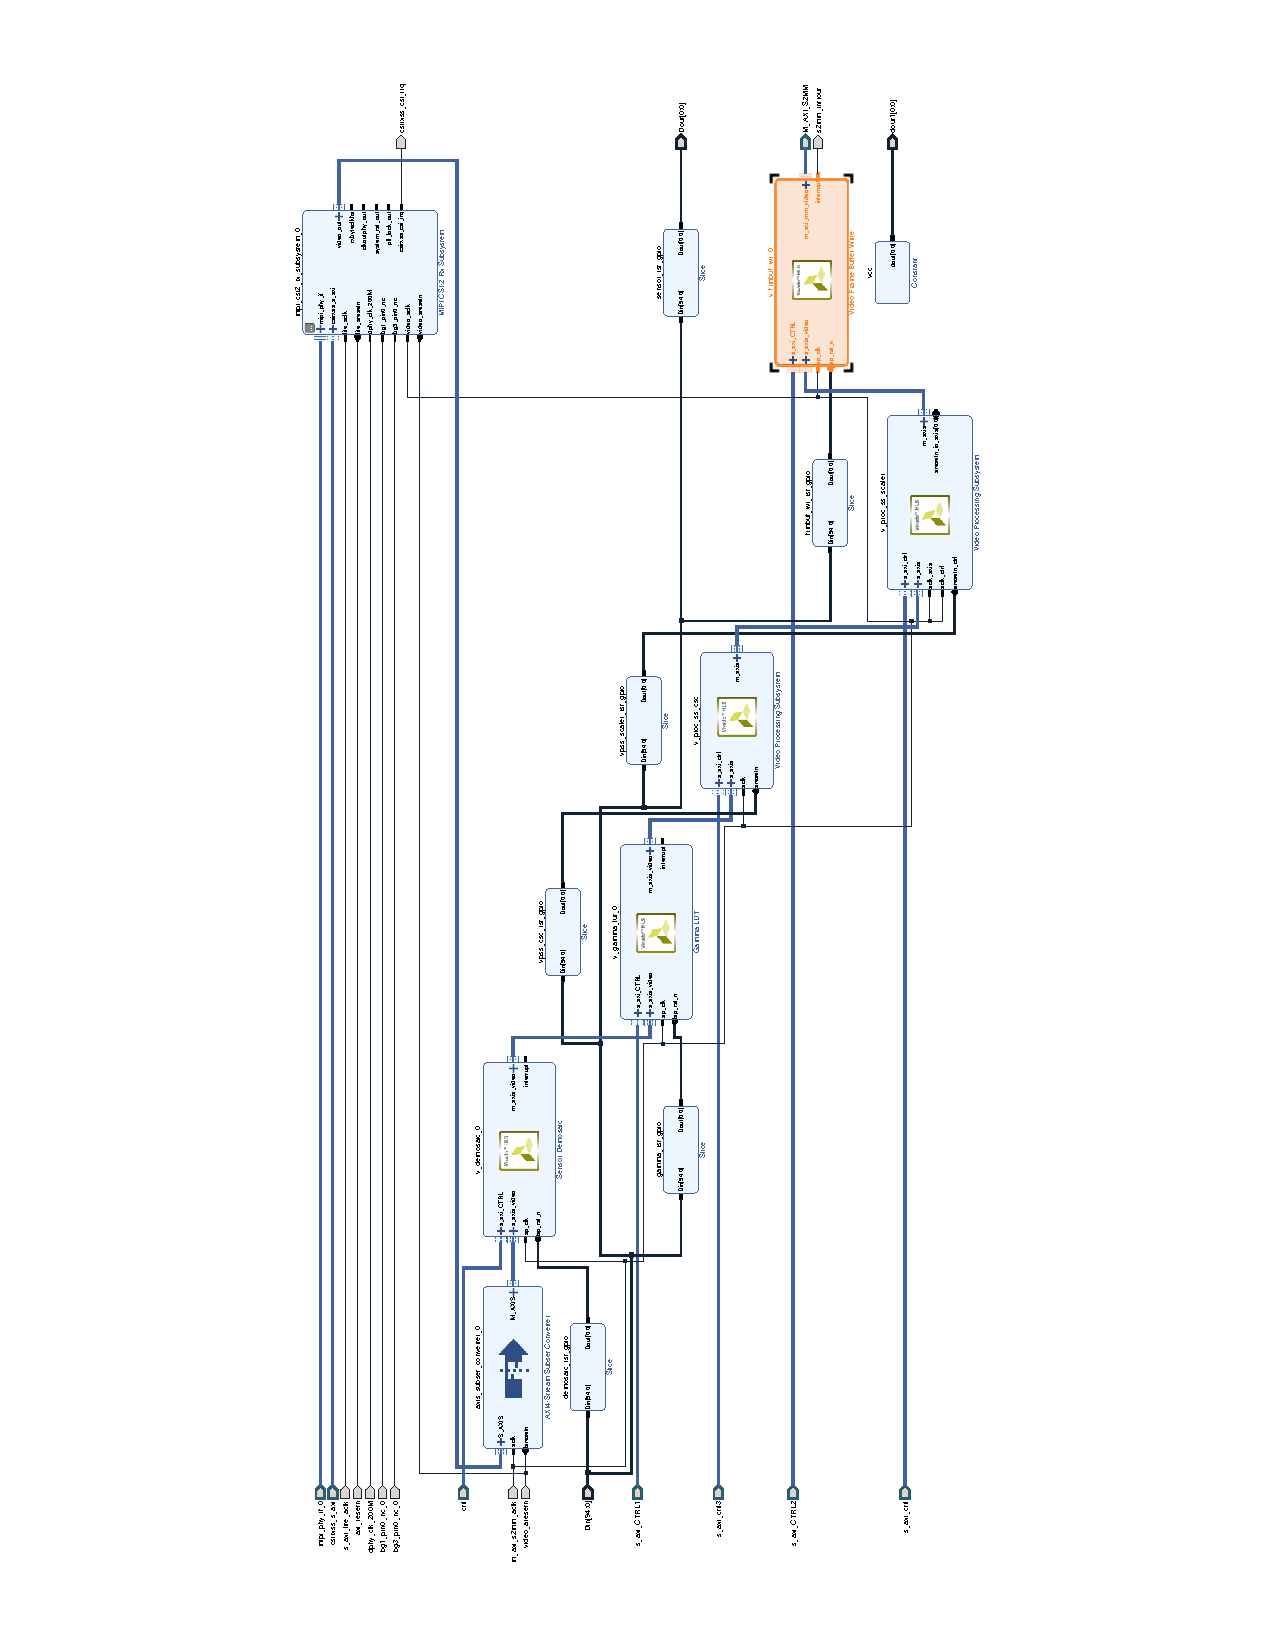
\includegraphics[width=\textwidth]{bilder/mipi_csi2_rx.pdf}
		\caption{\acs{MIPI} \acs{CSI} block design}
		\label{fig:mipi_block}
\end{figure}
Figure~\ref{fig:mipi_block} shows the reference design provided by Xilinx for the ZCU 104 board showing the complete hierarchy of the \ac{MIPI} \ac{CSI} block design with all additional blocks. These blocks are needed for further image processing. The data coming from the image sensor is in an unprocessed format called RAW. Therefore, an image processing pipeline needs to be integrated to convert this RAW image format into useable data in RGB format for example. The following Xilinx \acp{IP} are used to accomplish this task: 'Sensor Demosaic', 'Gamma LUT', 'Video Processing subsystem' and 'Video Frame Buffer Write'. The data transfer is handled by \ac{AXI} streaming interfaces.
Using the reference design as a starting point, the \ac{MIPI} subsystem was integrated into the hardware design together with the \ac{DPU} block. Afterward, Petalinux had to be configured and built. This enabled control of the whole system via an embedded Linux \ac{OS} host system running on the ARM cores. Several steps are necessary for setting up a Petalinux environment:
\begin{itemize}
	\item \textbf{Vivado hardware design:} First of all a working hardware design needed to be created in Vivado and successfully synthesized. This hardware design then needs to be exported in .hdf file format. This allows importing the hardware design as a template for the Petalinux system generation.
	\item \textbf{Creation of Petalinux project:} Petalinux is a command line tool for a Linux \ac{OS} which abstracts away some of the details of building an embedded Linux \ac{OS}. During generation of a new project, the previously used hardware design file is imported so that the system can access all of the implemented features.
	\item \textbf{Configuration:} In the next steps, necessary packages, user written apps, file system packages and custom modules can be added to the Petalinux project via console commands and a \ac{GUI} environment simplifying interaction with all of the possible options.
	\item \textbf{Building the system:} After all of the system is configured, the necessary packages and files need to be downloaded and a root file system and kernel image constructed. This can also be done via console commands. After successfully building the whole system the necessary files need to be generated for the system to boot. This includes a BOOT.bin file, an image.ub file and the root file system. These files and directories are the minimum necessities for the Petalinux \ac{OS}
\end{itemize}
To create a bootable image, an SD card is used and properly formatted. The SD card needs to partitioned into two primary partitions, BOOT formatted as FAT32 and ROOTFS, formatted as ext4. The Petalinux files are then copied over into the respective directories and the SD card can be used as the boot image for the \ac{FPGA} board.
\subsection{Synthara collaboration conference call}
Another Synthara conference call was due to further discuss details about the Embedded World 2019 demonstrator and a visit was organized to the company in order to create a schedule for the collaboration and labor division between Enclustra and Synthara.

\section{Week 9}
\subsection{Intel evaluation}
In this week a more closer evaluation of available neural network inference tools by Intel was done. The reason for this is the dependency solely on one \ac{FPGA} supplier is not ideal. In order to be flexible with product design and familiarity with all of the tools on the market for neural network inference, it was decided that some time should be spend on evaluating alternatives to Xilinx.
\begin{figure}[!htb]
	\centering
		\includegraphics[width=\textwidth]{bilder/openVINO-overview.png}
		\caption{OpenVINO toolkit overview~\cite{openvino}}
		\label{fig:openvino}
\end{figure}
Figure~\ref{fig:openvino} shows an overview over Intels OpenVINO toolkit. The workflow itself is similar to Xilinx \ac{DNNDK}. The starting point is a trained model using popular neural network training frameworks (Caffe, Tensorflow, etc.). The trained network is then passed to a model optimizer which performs tasks such as quantization, stripping away layers only needed for training and other tasks. This operation is hardware independent. An intermediate representation is generated and passed on to the inference engine. This is a high level \ac{API} allowing the implementation of neural networks on the target hardware. The main difference is its universal approach compared to the Xilinx \ac{DNNDK}. Intel acquired the \ac{FPGA} company Altera and took over their \ac{FPGA} modules. Therefore, the OpenVINO toolkit does not only support \acp{FPGA} but also all of other product families Intel offers, such as \acp{CPU}, \acp{GPU} as well as other more specialized hardware. One of the main problems with Intels offering is its support of only one \ac{FPGA} familiy, namely the Arria 10 \acp{FPGA}. Moreover, the model optimizer is not as powerful as the Xilinx \ac{DNNDK} one. No pruning is taking place and as of this date, there is no support for INT8 precision, only reduced precision floating point, which is not ideal. Therefore, the Xilinx approach is deemed superior.
\subsection{Petalinux workflow}
Integration and building of a custom Petalinux distribution continued this week with familiarizing myself with the overall workflow and possible debugging features. The \ac{DPU} \ac{IP} core was successfully integrated into the ZCU 104 reference design and synthesized. As the \ac{DNNDK} tool is still in a beta phase, there are frequent updates. A major update was released this week. This updated version was investigated and documented in the internal Enclustra Wiki. New sample applications were tested with the ZCU 104 evaluation board.

\section{Week 10}
\subsection{\acs{DNNDK} update}
In this week some further testing of the new \ac{DNNDK} version was done. The biggest change here is the added support for the Tensorflow framework. Tensorflow is the most popular neural network training framework right now as figure~\ref{fig:nnframeworks} shows. The x-axis represents the timeline and the y-axis is the percentage of frameworks mentioned in \ac{ML} publications.
\begin{figure}[!htb]
	\centering
		\includegraphics[width=\textwidth]{bilder/nnframeworks.jpg}
		\caption{Neural network framework usage overview \cite{frameworks}}
		\label{fig:nnframeworks}
\end{figure}
Although the output formats of Tensorflow are different than the Caffe output files, the work flow with the \ac{DNNDK} is basically the same as before: take the output of the framework, typically the trained weights and the network structure and feed it to the \ac{DNNDK} tools. Another big change is the separation between each of the tools provided by the \ac{DNNDK} package.
\begin{itemize}
	\item \textbf{\ac{IP} core:} \ac{DPU} \ac{IP} core to be integrated in hardware design
	\item \textbf{\ac{DNNDK} tools:} quantization and compression tools to acquire a binary file encapsulating the trained neural network model
	\item \textbf{\ac{AI} \ac{SDK}:} unified interface providing efficient implementations of common neural network layers as well as common neural networks (see figure~\ref{fig:ai_sdk})
	\begin{figure}[!htb]
		\centering
			\includegraphics[width=\textwidth]{bilder/ai_sdk.png}
			\caption{\ac{AI} \ac{SDK} overview \cite{ai_sdk}}
			\label{fig:ai_sdk}
	\end{figure}
\end{itemize}
\subsection{Petalinux workflow}
The Petalinux documentation was studied as well, especially setting up the device tree correctly. The device tree is a description of the hardware components that are present in a computer system so that the kernel can access these hardware components correctly. Part of this process is automated by the Petalinux tools, however, there are also manual additions that need to be added for the system to work as intended.
\subsection{Enclustra hardware integration}
After successfully integrating the \ac{DPU} \ac{IP} core into the ZCU 104 evaluation board the implementation of the \ac{DPU} on Enclustra modules was undertaken. Two different modules were chosen from the companies portfolio. One lower end ZYNQ Ultrascale device, the Mars XU3 and a higher end module, the Mercury+ XU1. The main difference concerning \ac{ML} performance is the number of \ac{DSP} blocks on the \acp{FPGA}. The \ac{DPU} can be instantiated in different sizes, the bigger the size the more performance. This is strongly dependent on the number of \ac{DSP} blocks that can be used. A comparison was made which sizes can be synthesized on these two modules. The much bigger Mercury+ XU1 can fit any of the available \ac{DPU} sizes (and has enough room for several instances of the \ac{DPU} \ac{IP} core) whereas the smaller Mars XU3 can only fit small \ac{DPU} sizes.

\section{Week 11}
\subsection{Enclustra hardware integration}
The \ac{DPU} integration into the reference designs available for the Mars XU3 and the Mercury+ XU1 continued in this week. For a successful integration the \ac{DPU} user guide was studied and the design adopted to the respective hardware platform. Figure~\ref{fig:dpu_hier} shows an overview over the \ac{DPU} subsystem.
\begin{figure}[!htb]
	\centering
		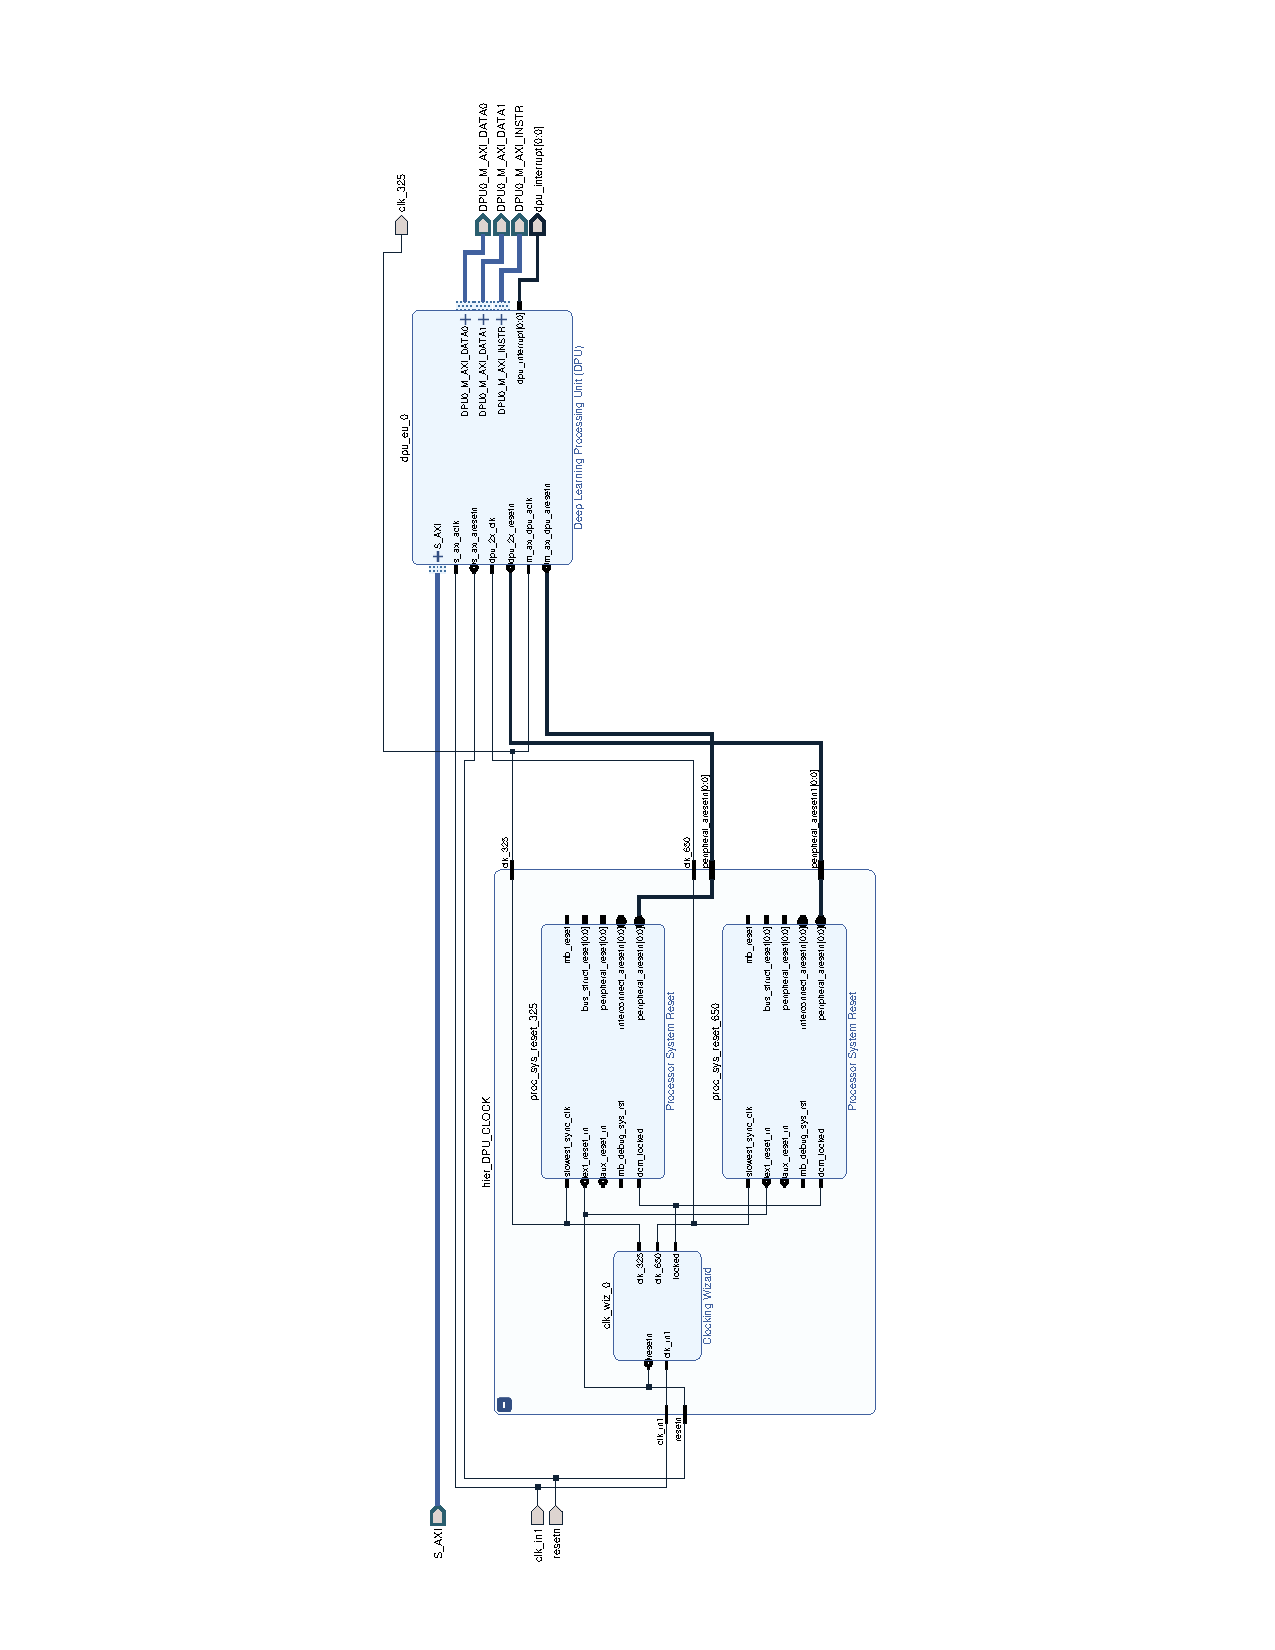
\includegraphics[width=\textwidth]{bilder/dpu_hier.pdf}
		\caption{\acs{DPU} hierarchy system}
		\label{fig:dpu_hier}
\end{figure}
Two main blocks comprise this subsystem: the clock generation and the \ac{DPU} \ac{IP} core itself. For generating the correct clock signals at appropriate frequencies a 'Clocking Wizard' \ac{IP} core is used. This block is configured to take an asynchronous reset and reference clock as input. Internally, a \ac{PLL} is used to generate faster clock frequencies which are needed for the \ac{DPU} \ac{IP} core. As this is a highly optimized hardware block, the frequency can be relatively high compared to the system block. In this design the \ac{DSP} slices are clocked with a frequency of 650 MHz. For each clock signal an asynchronous reset needs to be generated as well. This can be done via the 'Processor System Reset' \ac{IP} core. There, an asynchronous reset signal is generated for each respective clock domain. The data exchange of the \ac{DPU} \ac{IP} is handled by \ac{AXI} interfaces.
\subsection{Petalinux build}
The next part of the process is building the Petalinux image files. After extracting the hardware description file and building a Linux \ac{OS} the generated system can be simulated to verify correct functionality. The tool used for this is part of the Xilinx Petalinux tool flow called \ac{QEMU}. This tool is able of emulating a Xilinx ZYNQ system in software running on a Linux host system and offers some debugging tools. After some problems trying to emulate the kernel boot operation a Xilinx employee answered my forum question regarding my particular error message. As the \ac{DNNDK} is not yet fully released, \ac{QEMU} is not able to emulate the \ac{DPU}, which is not mentioned in the documentation of either tool.
\subsection{Synthara visit and collaboration discussion}
In this week on Thursday the visit to Synthara at ETH campus Irchel was scheduled and I went there with my supervisor Jelena and our marketing associate Melvin to discuss a possible collaboration in more detail. Synthara presented their rock-paper-scissors demonstrator and told us about their work flow which is quite similar to the Xilinx \ac{DNNDK}. They also presented their custom neural network used for the demonstrator, which is a very basic convolutional neural network. We agreed to developing a demonstrator together for Embedded World 2020 and made a project timetable. The work was separated among the different areas of expertise of each company with Synthara handling training the neural network and providing their custom neural network accelerator \ac{IP}. Enclustra would handle the necessary data collection and the hardware integration, both of which were my tasks.

\section{Week 12}
\subsection{Mars ST3 demonstrator}
This week the first samples of the Mars ST3 base board were available at the company after the usual bring up process for internal use. The bring up typically involves testing the hardware as thoroughly as possible and weed out errors in the \ac{PCB} design and the providing reference designs for the new board, which is compatible with all Mars \ac{FPGA} modules. My task was to make a small \ac{AI} demonstrator using this new base board and a Mars XU3 module. The reason for choosing the XU3 with the Zynq \ac{MPSoC} instead of the smaller Zynq 7000 \ac{SoC} was the compatibility of the Xilinx \ac{DPU} \ac{IP} core. The publicly released version was only suitable for Zynq Ultrascale devices. Support for Zynq 7000 \ac{SoC} would be added in a future release. I decided to port the \ac{DNNDK} sample applications to the Enclustra hardware. There were several reasons for this:
\begin{itemize}
	\item As the CEO of Enclustra would be attending a Xilinx conference in early June, having an \ac{AI} demonstrator to showcase would be great. This left only a few weeks for development.
	\item I was already familiar with the Xilinx \ac{DNNDK} work flow and due to the timing constraints this course of action was the most promising.
	\item No neural network needed to be trained as the already trained models from the \ac{DNNDK} can be used.
	\item The necessary hardware integration was completed successfully in the previous weeks for the XU3 module and therefore could be used for porting the sample applications to the complete hardware design with the new Mars ST3 board.
\end{itemize}
The main difficulty was posed by the Petalinux implementation as there are no official guidelines by Xilinx for custom boards. However, the official Xilinx tutorial found at \href{https://github.com/Xilinx/Edge-AI-Platform-Tutorials/tree/master/docs/DPU-Integration}{https://github.com/Xilinx/Edge-AI-Platform-Tutorials/tree/master/docs/DPU-Integration} provides an excellent starting point for custom projects. After a few adjustments to the device tree specific to the Enclustra hardware and Petalinux configuration adjustments for the exported .hdf file, the resnet50 image classification application was successfully running on the Enclustra hardware. The setup is shown in figure~\ref{fig:st3_demo_resnet}.
\begin{figure}[!htb]
	\centering
		\includegraphics[width=\textwidth]{bilder/placeholder.png}
		\caption{resnet50 demonstrator overview}
		\label{fig:st3_demo_resnet}
\end{figure}
This first version of the demonstrator consists of a \ac{DP} monitor, the Mars ST3 base board, the Mars XU3 module and a serial connection to control the application via terminal from the host PC (adding keyboard and mouse to the \ac{FPGA} module itself would make this step obsolete).
A toggle button was implemented to allow switching between two modes, going through the data set one by one or classifying all images in the data set as fast as possible. One mode is to show the correct result of the classification as otherwise the classification is too fast to observe by eye. The other mode is to show the classification speed. An example for this can be seen in figure~\ref{fig:resnet_classification}.
\begin{figure}[!htb]
	\centering
		\includegraphics[width=\textwidth]{bilder/placeholder.png}
		\caption{resnet50 classification example}
		\label{fig:resnet_classification}
\end{figure}

\section{Week 13}
\subsection{Mars ST3 demonstrator preparation}
The deadline to finish the \ac{AI} demonstrator was this week Tuesday. So in the beginning of the week I worked on polishing the resnet50 example to have a smooth demo application. Furthermore, the face detection demo was also ported to the Enclustra hardware. The camera used was the same one from the Xilinx evaluation kit. A \ac{USB} 3.0 3.4 MP camera module. The reason for using the \ac{USB} camera for the demonstrator again was due to the strict timing constraints for the project. Furthermore, the camera used utilizes the standard V4L2 Linux kernel driver. This enables plug and play of the camera module and auto detection of the Petalinux \ac{OS}. Therefore, no additional driver needed to be written. The applications were written using the Xilinx \ac{SDK} against the exported root file system and libraries from the Petalinux build. In order to have access to all of the necessary functions of the \ac{DNNDK} the correct Linker flags and environmental variables needed to be set. Additionally, the utilized libraries needed to be specified. The resnet50 application and the face detection application have different requirements of course, so two applications have been implemented with the \ac{SDK}. The output of the \ac{DNNDK} compiler was included as well into the project. These output binary files are the result of the neural network compilation containing the neural network model. Compiling the whole application combines these \ac{DNNDK} binary files with the application binary file into a hybrid binary file, that can be used to run the application. Pose detection as a third demonstration application was also started to be implemented but ultimately forfeited due to the limited time. Consequently, the demonstrator has two sample applications, image classification using resnet50 and face detection, running on Enclustra hardware. All the project files and scripts necessary to replicate the design have been collected and documented for re-usability.
\subsection{ROCK-PAPER-SCISSOR demonstration data collection preparation}
The second part of the week was used to prepare the data collection for the rock-paper-scissors demo. After the Synthara visit the information of how to obtain a good quality data set were shared and it was my task to create the setup for the data collection. First of all, the number of classes needed to be defined: There was one class for each of the correct symbols (rock, paper, scissors), one illegal symbol class and one background class, resulting in a total of five classes. Figure~\ref{fig:dataset_overview} summarizes the data set structure and points out the requirements for a good quality data set.
\begin{figure}[!htb]
	\centering
		\includegraphics[width=\textwidth]{bilder/dataset_overview.png}
		\caption{Data set overview and requirements for a good quality data set}
		\label{fig:dataset_overview}
\end{figure}

\section{Week 14}
\subsection{ROCK-PAPER-SCISSOR demonstration data collection preparation}
The need for a quality data set and the amount of data that needed to be collected made automation of the process necessary to speed things up. The hardware that we wanted to use for the demonstrator was the Mars XU3 module and the Mars ST3 base board. Furthermore, the RPi camera utilizing a \ac{MIPI} connector was to be used. The easiest way to obtain the necessary amount of data (about 10k pictures in total) needed was to use the Raspberry Pi together with the camera. The operating system on the Raspberry Pi provides all the functions to obtain videos quickly and extract frames from videos. For the collection of a good quality data set variation is key. Therefore, the contribution of as many people as possible is necessary. The setup for collecting the data set looked as follows:
\begin{itemize}
	\item take videos of each subject
	\item 150 seconds per symbol per subject
	\item extract frames from the video
	\item structure the data so it gets labeled directly (ROCK, PAPER, SCISSORS, ILLEGAL)
\end{itemize}
\subsection{Shell scripting and presentation on data set collection}
To automatize this process, a shell script was written handling all of the tasks mentioned above. The script generates the necessary folder structure, takes the video and saves it. A conversion from .h264 to .mp4 format is done to easier extract the frames from the video. After discussing the frame size with Synthara, a video resolution of 320x240 with a framerate of 60 fps was chosen. This is the lowest resolution supported by the camera drivers for the Raspberry Pi.
The test setup was build up in the kitchen area, so as to get as many people as possible to contribute to the data set collection. In order to have everybody know what to do, a short presentation was prepared to inform the colleagues of the purpose of this data set collection and also the procedure. Details were given about what constitutes a quality data set and how to obtain it. Emphasis was laid upon how to move the subjects hand and arm in order to generate useful data. Emphasis was laid on not moving the hand out of the camera frame, as this would generate a lot of falsely labeled data, which in turn degrades the network performance during training significantly. A diagram of the data collection setup is shown in figure~\ref{fig:setup}.
\begin{figure}[!htb]
	\centering
		\includegraphics[width=\textwidth]{bilder/placeholder.png}
		\caption{Data set collection setup}
		\label{fig:setup}
\end{figure}

\section{Week 15}
\subsection{Data set collection}
The majority of this week was spent collecting the data set. Therefore, the data collection setup was build up in the kitchen area and various employees were asked to participate. I went from one to the after I was done with one subject. A total of 10 minutes per subject of data was captured via video. As mentioned before, a Raspberry Pi was used with the script I created to collect the data and automatize as much of the process as possible. During the data set collection I assisted in keeping the movements of the subject in check and talk them through the collection process. For each of the symbols (ROCK, PAPER, SCISSORS, ILLEGAL) a video of 150 seconds was recorded. After each symbol, a short break was incorporated, as this seemingly small time period already puts a strain on the arm. This process was repeated for any employee that was available. A monitor was used to directly show the camera video feed so that the position of the hand within the frame was visible and could be easily corrected.
\subsection{Intel \acs{ML} seminar in Lausanne}
On Wednesday, I traveled to Lausanne to attend an Intel seminar on \ac{AI} inference with Intel products. The main reason for going to this event was to acquire more knowledge of the OpenVINO toolkit for \ac{FPGA}. In addition, a block of the seminar dealt with data set preparation and augmentation for training neural networks. One of the key methods to create the necessary amount of data is data augmentation. This can be described as oversampling the data set, basically creating more data from existing data by rotating, shifting, zooming and other image manipulations. In this way, the data set can be evenly balanced as well so that each class has a similar amount of images. The data set is then separated into three subsets:
\begin{itemize}
	\item training set: data used to train the network
	\item validation set: subset of the test set used for hyperparameter tuning (learning rate, momentum, etc.)
	\item test set: data that the network has not seen during training, which is used for a full evaluation of the performance of the network
\end{itemize}
The data augmentation process only applies to the training set. As to new information regarding the OpenVINO toolkit, there was no additional information given as to what is available online. Overall, the focus was not on \ac{FPGA} programming. The main idea of Intel is to provide a unified platform to develop \ac{AI} applications using OpenCL and then provide plugins to optimize the device independent code for the individual hardware, like \acp{FPGA}.
\begin{figure}[!htb]
	\centering
		\includegraphics[width=\textwidth]{bilder/placeholder.png}
		\caption{Something}
		\label{fig:something}
\end{figure}
The rest of the week was spent collecting more data from Enclustra employees with the created data collection setup.

\section{Week 16}
\subsection{Data set collection}
The final data set collection amounted to 11503 images with a distribution of 2838 images for the 'ROCK' class, 2820 images for the 'PAPER' class, 2814 images for the 'SCISSORS' class and 2749 images for the 'ILLEGAL' symbol class. The 'BACKGROUND' class consists of 282 images. To add to this number a publicly available data set was also added to the collection containing 2188 images in total distributed almost equally amongst the classes 'ROCK', 'PAPER' and 'SCISSORS'. The complete data set was then handed of to Synthara for the training process as agreed when starting the collaboration. The data set was augmented as described in the chapter before and then iteratively quantized to compress the network.
\subsection{Robot hand ordering}
As the training process would take up to two weeks at least, the next reasonable step was to work on the hardware setup with the Enclustra board. A crucial part for this is the robotic hand. At first, I conducted research into the available possibilities: There are numerous options ranging from cheap ($\sim 50$ \$) servo motor controlled basic hands to more sophisticated 3D-printed medical variants (several thousand \$). For this demonstrator the key parameter was speed, so that the robot hand would react in time to the classification results provided by the neural network. The key parameter for this is how quickly the attached servos can go from 0 $^\circ$ to 180 $^\circ$. The typical value for this is around 1 to 2 $ms$ for the cheaper robotic hands. The more expensive 3D printed ones were taken out of consideration because of the cost.
\begin{figure}[!htb]
	\centering
		\includegraphics[width=0.5\textwidth]{bilder/robohand.jpg}
		\caption{Robotic hand chosen for the demonstrator}
		\label{fig:robohand}
\end{figure}
Figure~\ref{fig:robohand} shows the chosen robotic hand. The benefits of this system is the added \ac{PCB} together with a microcontroller, so that the basic functionality can be tested easily and directly. The servos used in this hand are very standard servo motors with three connectors, VCC, GND and DATA. The DATA line is used to determine the angle which the servo has to drive to. The signal used for this is a \ac{PWM}. Figure~\ref{fig:pwm_servo} shows the mapping of the \ac{PWM} signal to the motor position.
\begin{figure}[!htb]
	\centering
		\includegraphics[width=0.5\textwidth]{bilder/pwm.png}
		\caption{\acs{PWM} signal servo motor position mapping}
		\label{fig:pwm_servo}
\end{figure}
\subsection{Internship documentation}
The rest of the week was spent on writing documentation of all of the tasks I completed during my internship so far and integrate this information into the company Wiki.